\documentclass[14pt]{extarticle}
\usepackage[utf8]{inputenc}
\usepackage[T1]{fontenc}
\usepackage[spanish,es-lcroman]{babel}
\usepackage{amsmath}
\usepackage{amsthm}
\usepackage{physics}
\usepackage{tikz}
\usepackage{float}
\usepackage[autostyle,spanish=mexican]{csquotes}
\usepackage[per-mode=symbol]{siunitx}
\usepackage{gensymb}
\usepackage{multicol}
\usepackage{enumitem}
\usepackage[left=2.00cm, right=2.00cm, top=2.00cm, 
     bottom=2.00cm]{geometry}

%\renewcommand{\questionlabel}{\thequestion)}
\decimalpoint
\sisetup{bracket-numbers = false}

\title{\vspace*{-2cm} Práctica 5 - Principio de Bernoulli y Torricelli \\  Física IV (Área II) \vspace{-5ex}}
\date{}

\begin{document}
\maketitle

\section{Datos para la práctica.}

\begin{itemize}
\itemsep0em 
\item  \textbf{Práctica:} 5.
\item \textbf{Unidad:} Dos.
\item \textbf{Temática:} Hidrodinámica.
\item \textbf{Nombre de la práctica:} Principio de Bernoulli y Torricelli.
\item \textbf{Número de sesiones que se requieren para la práctica:} Tres.
\item \textbf{Objetivo general: } Determinar de manera experimental la velocidad de salida de un fluido que circula a través de un orificio de un envase a partir de la altura, así como el alcance del chorro como función de la velocidad y tiempo de vaciado.
\item \textbf{Hipótesis: } El chorro de agua que sale  por la marca a mayor distancia de la superficie tiene la mayor velocidad y el mayor alcance. 
\end{itemize}

\textbf{Planteamiento del problema:} 

La hidrodinámica es el estudio de las propiedades mecánicas y los fenómenos que presentan los fluidos en movimiento.

\textbf{Ecuación de Bernoulli.}

Las leyes de la dinámica para cuerpos sólidos (recordemos que la dinámica se enfoca en estudiar el movimiento de los objetos atendiendo la causa que los origina), son aplicables también a los fluidos, es decir, a líquidos y gases. Debido a que éstos no tienen forma propia, sino la del recipiente que los contiene, se hacen las consideraciones como si fuesen fluidos ideales.

Daniel Bernoulli (1700-1782), físico suizo, estudió el comportamiento de los líquidos y aplicó precisamente una de estas leyes: la ley de conservación de la energía, al comportamiento de un líquido en movimiento.

Los resultados de los estudios de Bernoulli se pueden resumir así:

\begin{enumerate}
\item La presión que ejerce un líquido que fluye por un conducto es mayor cuando el líquido fluye a bajas velocidades, y menor cuando aumenta la velocidad de flujo.

Es decir, cuando las líneas de flujo se aproximen entre sí, la presión en dicha región será menor.
\item En un líquido ideal cuyo flujo es estacionario, la suma de las energías cinética, potencial y de presión que ejerce un líquido se mantiene constante, es decir, la suma de estas energías en un punto determinado, es igual a la suma de dichas energías en cualquier otro punto.
\end{enumerate}

\textbf{Teorema de Torricelli.}

La ecuación de Bernoulli puede ser aplicada para obtener la velocidad de salida de un líquido contenido en un recipiente, al cual se le hace un orificio en algún punto por debajo del nivel al que se encuentra la superficie libre del fluido.

Lo que nos explica el Teorema de Torricelli es: \enquote{La velocidad con la que un líquido sale por un orificio de un recipiente, es igual a la que adquiriría un cuerpo que se dejara caer libremente desde la superficie libre del líquido, hasta el nivel en que se encuentra el orificio}.

Es decir, la velocidad de salida de un líquido depende de su densidad y de la altura o profundidad a la que se encuentra el orificio de salida.

\section{Marco teórico.}

Para elaborar el marco teórico, responde las siguientes preguntas, en caso de que requieras apoyarte con una expresión (fórmula) deberás de explicar cada elemento o componente de la misma.

\begin{enumerate}
\item ¿Qué nos explica la ecuación de continuidad en un fluido?
\item ¿Cuál es la ecuación de Bernoulli?
\item ¿Por qué la ecuación de Torricelli es un caso especial de la ecuación de Bernoulli?
\item ¿Por qué un avión que pesa en promedio $200$ toneladas puede volar?
\end{enumerate}

\section{Material.}

\begin{enumerate}[label=\roman*)]
\item 1 envase vacío de tetrapack (o un envase de PET) de 1.5 o 2 litros.
\item 1 clavo.
\item Tijeras o cutter.
\item Cinta masking tape o barra de plastilina.
\item Regla o flexómetro.
\item Agua.
\end{enumerate}

\subsection{Procedimiento.}

\begin{enumerate}
\item Con mucho cuidado recorta la parte superior del envase, de tal manera que tengas solo la parte ya sea rectangular o circular.
\item Mide el largo de una cara lateral del envase. Anota el valor: \rule{2cm}{0.1mm}
\item Distribuye 3 marcas espaciadas de manera uniforme sobre la cara lateral.
\item A partir de la parte superior del envase, mide la distancia que tiene cada marca.
\begin{figure}[H]
    \centering
    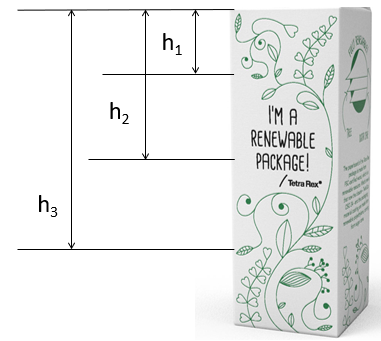
\includegraphics[scale=1]{Imagenes/Practica_04_Tetrapack_01.png}
\end{figure}
\item Con el clavo, perfora la cara del envase en cada marca.
\item Con masking tape, cinta adhesiva o plastilina cubre las tres marcas.
\item Agrega agua al envase hasta la parte superior.
\item Se va a registrar el \enquote{alcance} del chorro de agua que sale de cada marca, para ello, acondiciona la regla o flexómetro en la parte inferior de la mesa para medir la distancia que se tiene del envase al punto donde cae el agua sobre la horizontal. Se recomienda que el chorro de agua caiga en la tarja para evitar derrames o salpicaduras.
\item Con cuidado retira la cinta o plastilina de la primera marca.
\item Registra el tiempo que tarda el agua en vaciarse por la primera perforación, es decir, la que está en $h_{1}$, anota el valor en la tabla.
\item Registra la distancia $d_{1}$ que alcanza el chorro en la marca, anota el valor en la tabla.
\begin{figure}[H]
    \centering
    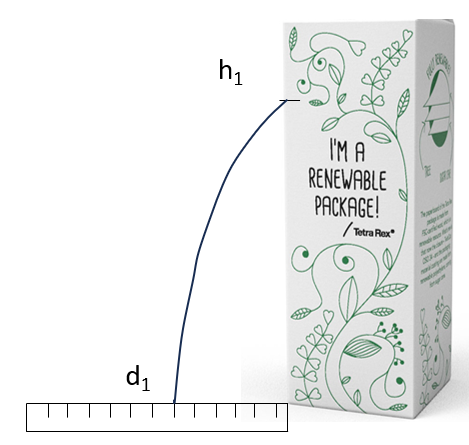
\includegraphics[scale=1]{Imagenes/Practica_04_Tetrapack_02.png}
\end{figure}
\item Una vez que ya no sale agua de la marca, tapa la misma y agrega nuevamente agua al envase hasta llenarlo.
\item De manera cuidadosa, repite este procedimiento para las otras dos marcas, anotando los tiempos en la tabla, así como la distancia de los chorros.
\end{enumerate}

\begin{table}[H]
    \centering
    \begin{tabular}{| c | c | c | c |} \hline
        Marca & Altura [\unit{\meter}] & Tiempo [\unit{\second}] & Distancia [\unit{\meter}] \\ \hline
        $h_{1}$ & & & \\ \hline
        $h_{2}$ & & & \\ \hline
        $h_{3}$ & & & \\ \hline
    \end{tabular}
\end{table}

\end{document}